\documentclass[a5paper]{article}
\usepackage[a5paper, top=8mm, bottom=8mm, left=8mm, right=8mm]{geometry}

\usepackage{polyglossia}
\setdefaultlanguage[babelshorthands=true]{russian}

\usepackage{fontspec}
\setmainfont{FreeSerif}
\newfontfamily{\russianfonttt}[Scale=0.7]{DejaVuSansMono}

\usepackage[font=scriptsize]{caption}

\usepackage{amsmath}
\usepackage{amssymb,amsfonts,textcomp}
\usepackage{color}
\usepackage{array}
\usepackage{hhline}
\usepackage{cite}
\usepackage{verse}
\usepackage{xcolor}

\usepackage[hang,multiple]{footmisc}
\renewcommand{\footnotelayout}{\raggedright}

\PassOptionsToPackage{hyphens}{url}\usepackage[xetex,linktocpage=true,plainpages=false,pdfpagelabels=false]{hyperref}
\hypersetup{colorlinks=true, linkcolor=blue, citecolor=blue, filecolor=blue, urlcolor=blue, pdftitle=1, pdfauthor=, pdfsubject=, pdfkeywords=}

\usepackage{tabu}

\usepackage{graphicx}
\usepackage{indentfirst}
\usepackage{multirow}
\usepackage{subfig}
\usepackage{footnote}
\usepackage{minted}

\newcommand{\attribution}[1] {
    \vspace{-5mm}\begin{flushright}\begin{scriptsize}\textcolor{gray}{\textcopyright\, #1}\end{scriptsize}\end{flushright}
}

\sloppy
\pagestyle{plain}

\title{Лекция 14: Развёртывание}
\author{Юрий Литвинов\\\small{yurii.litvinov@gmail.com}}
\date{30.05.2022}

\begin{document}

\maketitle
\thispagestyle{empty}

На этой лекции поговорим о более практических вещах: о том, как и куда развёртывать приложение.

\section{Docker}

Концептуально Docker --- это легковесная виртуальная машина, которая виртуализирует не машинные команды, как обычные виртуалки, а системные вызовы, то есть используется ядро операционной системы машины-хоста. Что хуже в плане изоляции, чем обычные виртуалки (например, вирусы в Docker-контейнерах запускать может быть плохой идеей), но гораздо быстрее. Ещё Docker-контейнеры отличаются от виртуалок тем, что в них работает один процесс. В принципе, это легко обойти, но концептуально контейнер --- это виртуализированный процесс, а не виртуализированная машина:

\begin{center}
    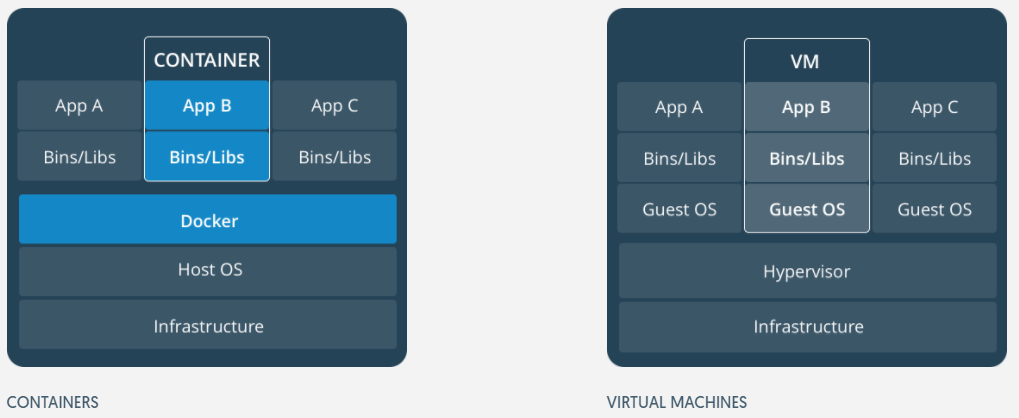
\includegraphics[width=0.7\textwidth]{docker.png}
    \attribution{\url{ https://www.docker.com}}
\end{center}

Docker-образы (то есть то, из чего запускаются контейнеры) только для чтения, то есть чтобы хранить в контейнере какие-то данные, надо отобразить его файловую систему на файловую систему хостовой машины. Тем не менее, Docker --- это стандарт де-факто по деплою распределённых приложений, потому что позволяет запустить готовое к работе приложение буквально одной командой. 

Поскольку Docker используется практически повсеместно, довольно прост в настройке и использовании, и обеспечивает массу преимуществ, крайне рекомендую использовать его уже сейчас, для своих проектов. Если они связаны с веб --- то однозначно, если это что-то консольное --- тоже очень желательно (для того, чтобы каждый мог собрать и запустить, без установки правильных версий компилятора и всех библиотек), если с графическим интерфейсом --- сложнее, но можно. Под Linux Docker поставить и настроить очень просто, под Windows, возможно, придётся повозиться --- если сделать это неправильно, он будет запускать VirtualBox, то есть настоящую виртуалку. Если сделать это правильно, придётся ставить WSL2 (к счастью, в Windows 11 она вроде как уже установлена) и терпеть исчезновение примерно 35 Гб места на диске. И ещё, возможно, включить HyperV в настройках BIOS (который давно уже называется UEFI, но традиции сильны), но это уж как повезёт.

Помимо самого Docker есть ещё Docker Desktop --- красивый UI для управления Docker, контейнерами и образами, и Docker Hub --- репозиторий для образов, наподобие GitHub и столь же бесплатный (причём, в отличие от Docker Desktop, бесплатный даже для коммерческих применений, хотя и с некоторыми квотами). Поскольку Docker --- стандарт де-факто, его знают и умеют с ним работать все нормальные оркестраторы и облачные провайдеры.

Docker-образ (Docker Image) --- это запускабельный образ приложения со всем окружением, необходимым ему для работы (можно понимать как очень навороченный .exe-файл). Образ состоит из слоёв, доступных только для чтения. Например, поверх слоя Alpine Linux лежит слой рантайма ASP.NET, поверх которого слой вашего веб-сервиса, поверх которого лежит слой конфигурации:

\begin{center}
    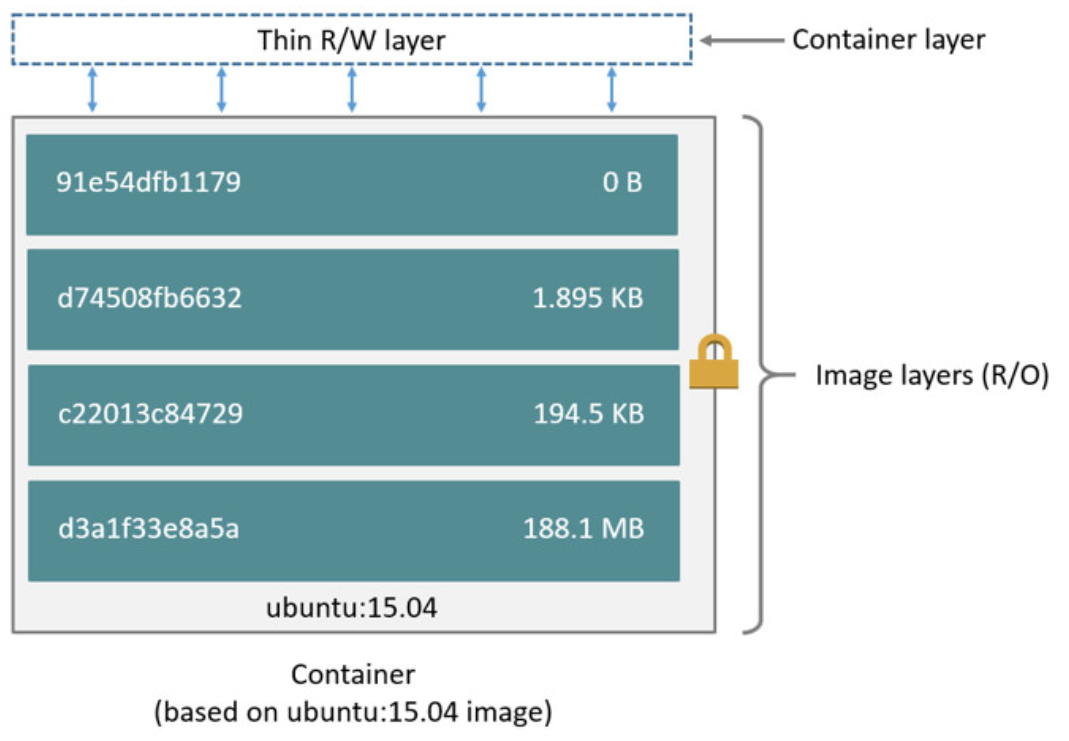
\includegraphics[width=0.5\textwidth]{dockerLayers.png}
    \attribution{\url{ https://www.docker.com}}
\end{center}

Каждый слой имеет свою файловую систему и свои переменные окружения, и результирующая файловая система образа получается просто накладыванием слоёв последовательно один на другой (то есть если в слое A есть file1.txt и file2.txt, а в слое B file2.txt и file3.txt, в результирующем образе будет три файла). Поскольку слои read-only, образы могут разделять слои между собой, как процессы могут разделять динамические библиотеки. Так что, например, если у вас на машине 20 образов поверх Alpine Linux, то слой Alpine Linux у вас ровно один, что очень позитивно сказывается на объёме хранимых данных и потребляемом сетевом трафике (образы скачиваются послойно, так что если вы скачали слой один раз, он больше не качается).

Любой образ может служить базой для создания другого образа. Это, собственно, обычно и делается, когда вы собираете свой образ --- поверх всех слоёв существующего образа кладёте один или несколько своих слоёв.

Docker-контейнер (Docker Container) --- это запущенный экземпляр образа, типа запущенного .exe-файла:

\begin{center}
    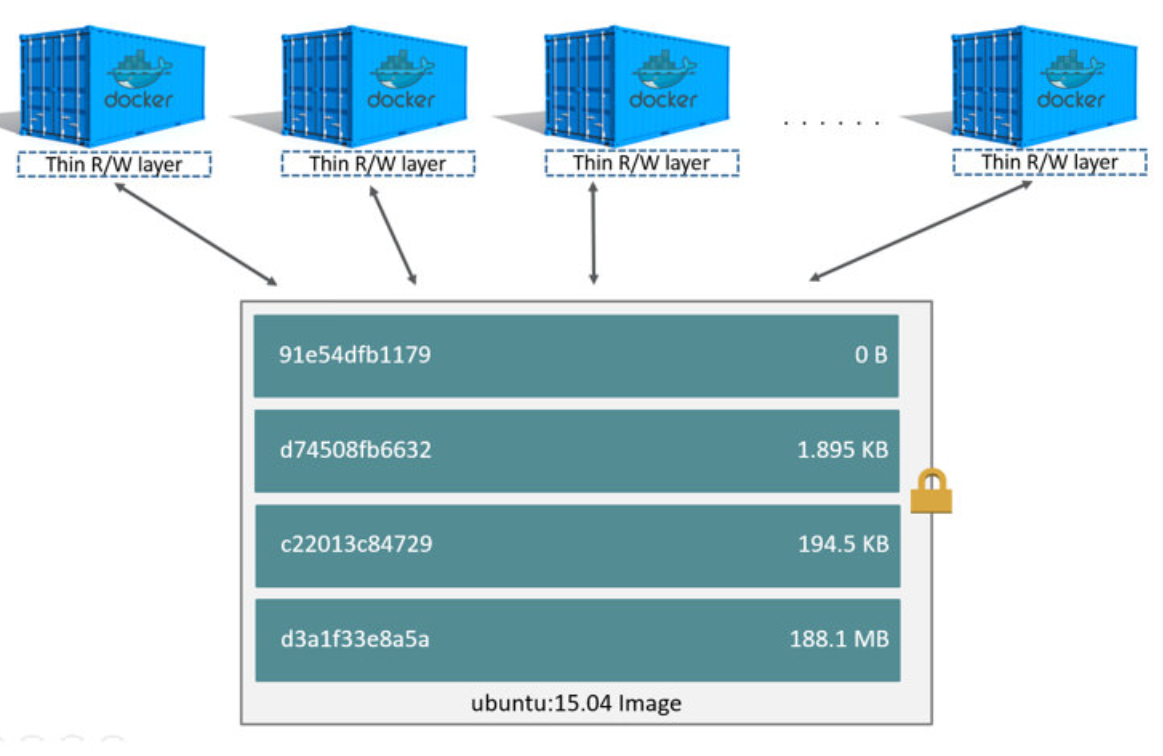
\includegraphics[width=0.6\textwidth]{dockerContainer.png}
    \attribution{\url{ https://www.docker.com}}
\end{center}

У контейнера есть дополнительный слой для записи, который может использоваться файловой системой внутри контейнера для хранения временных данных, но все изменения в нём гибнут при перезапуске контейнера (однако можно сохранить контейнер с его текущим состоянием файловой системы как новый образ). Контейнер содержит один запущенный процесс. Ничто не мешает этому процессу быть, например, bash, но обычно в контейнере работает просто целевое приложение.

Docker Hub\footnote{\url{https://hub.docker.com/} (дата обращения: 12.12.2021).} --- это централизованный репозиторий Docker-образов, куда выкладывают образы все приличные разработчики, включая официальные образы различных дистрибутивов и образы, собранные обычными пользователями. Обычно выкладываемые туда образы публичны, но за небольшие деньги можно получить приватные репозитории плюс доступ к CI/CD для сборки образов (не то чтобы это сильно надо, образы можно собирать любой CI-системой, хоть GitHub Actions, но на Docker Hub может быть гораздо быстрее). В принципе, Docker Hub --- это не единственный репозиторий образов, GitHub имеет свой (там образы по умолчанию приватные и их даже не так просто сделать публичными), большие облачные провайдеры имеют свой (Amazon Elastic Container Registry, Azure Container Registry, например), можно поднять свой (из официального Docker-образа, лежащего на Docker Hub). Однако Docker Hub используется по умолчанию (так же, как GitHub --- стандарт де-факто для git-репозиториев, хотя есть несколько хороших альтернатив и ничто не мешает поднять свой, даже с красивым графическим интерфейсом --- см. GitLab).

\subsection{Технические детали}

Собственно, предположим, что вы установили себе Docker. Что-то поделать с ним можно через Docker Desktop или вашу любимую среду разработки (скорее всего, она много чего умеет), но вообще docker --- это консольная утилита (даже две, docker daemon, запускающийся как сервис, и docker, консольный клиент для него). Вот самые основные команды:

\begin{itemize}
    \item docker run --- запускает контейнер. Если такого контейнера нет, делает pull, по умолчанию с Docker Hub. Основные аргументы:
    \begin{itemize}
        \item -d --- запустить в фоновом режиме. Без этого ключа docker не вернёт управление, пока контейнер не закончит работу, что может быть хорошо для отладки, но в боевом режиме не нужно;
        \item -p host\_port:container\_port --- прокинуть порт из контейнера на хост. Поскольку образы read-only, приложения в них сконфигурированы под некую абстрактную машину так, будто они на ней одни (например, слушают порт 80). Если запускаете два контейнера, каждый из которых слушает порт 80, случилась бы беда, поэтому docker сам симулирует сетевой стек и отображает порты хоста на порты контейнера в момент запуска контейнера. Так что какой порт выделить контейнеру, решает админ хоста, а не автор образа. По умолчанию все порты в контейнере закрыты, так что без ключа -p сетевое приложение запускать просто нет смысла.
        \item -i -t --- запустить в интерактивном режиме. Если в контенйере есть терминал, можно запустить его в интерактивном режиме, весь ввод с клавиатуры будет передаваться терминалу, а весь вывод --- вам в консоль, так что можно работать в контейнере так, будто вы подключились к удалённой машине по SSH. Очень удобно для отладки, но вручную что-то конфигурировать так в контейнере --- плохая идея, при перезапуске все изменения пропадут
        \item Пример: \mintinline{text}|docker run -it ubuntu /bin/bash|
    \end{itemize}
    \item docker ps --- показывает запущенные сейчас на хосте контейнеры с их id-шниками, по которым им можно потом посылать команды. Например, \mintinline{text}|docker run -d nginx; docker ps|
    \item docker stop --- останавливает контейнер (на самом деле шлёт SIGTERM, затем SIGKILL процессу в контейнере --- приложение внутри вправе проигнорировать эти сигналы);
    \item docker exec --- запускает дополнительный процесс в уже запущенном контейнере (если он там есть). В контейнеры очень редко ставят полноценный Linux с Bash, потому что они довольно большие, но есть набор утилит BusyBox, который словно бы создан для ручного ковыряния в контейнере --- размером он чуть более 2 мегабайт, но реализует все основные утилиты Unix, включая ash (Almquist Shell, легковесный, но не очень функциональный аналог bash). Поэтому если предполагается, что надо будет ходить внутрь контейнера, добавить туда слой с BusyBox может быть хорошей идеей.
\end{itemize}

\subsection{Dockerfile}

Чтобы собрать свой образ, потребуется Dockerfile --- это конфиг сборки контейнера, типа Makefile для Docker. Вот самый простой пример, из документации:

\begin{minted}{sh}
# Use an official Python runtime as a parent image
FROM python:2.7-slim

# Set the working directory to /app
WORKDIR /app

# Copy the current directory contents into the container at /app
ADD . /app

# Install any needed packages specified in requirements.txt
RUN pip install --trusted-host pypi.python.org -r requirements.txt

# Make port 80 available to the world outside this container
EXPOSE 80

# Define environment variable
ENV NAME World

# Run app.py when the container launches
CMD ["python", "app.py"]
\end{minted}

Команда FROM задаёт, на базе какого образа строится новый образ. Имя образа --- это собственно его имя, и \emph{тэг} после двоеточия. Тэг в принципе может быть любой строкой, но обычно используется \emph{semantic versioning} или специальные тэги типа latest.

WORKDIR --- это папка в файловой системе контейнера, которая будет рабочей для запускаемого процесса. 

ADD рекурсивно копирует содержимое указанной папки на хосте в файловую систему контейнера (тут мы копируем всю папку, где лежит Dockerfile, в папку /app в контейнере --- да, прямо в корень файловой системы, всё равно она больше никому, кроме нашего приложения, не будет видна).

RUN исполняет при сборке образа указанную команду. Тут мы менеджером пакетов Python ставим зависимости, которые заранее указали в requirements.txt.

EXPOSE открывает порт в контейнере (открываем порт 80).

ENV определяет переменную окружения, которая будет установлена в контейнере (самый простой способ управлять конфигурацией контенйера, благо переменные окружения можно переопределить при запуске).

Ну и последняя команда --- CMD, определяет, что надо запускать при старте контейнера. Тут запускается интерпретатор Python на указанный скрипт (из WORKDIR).

Вот несколько более интересный пример, типичного Dockerfile для типичного ASP.NET-приложения:

\begin{minted}{docker}
FROM mcr.microsoft.com/dotnet/aspnet:6.0 AS base
WORKDIR /app
EXPOSE 80
EXPOSE 443

FROM mcr.microsoft.com/dotnet/sdk:6.0 AS build
WORKDIR /src
COPY ["ConferenceRegistration/ConferenceRegistration.csproj", "ConferenceRegistration/"]
RUN dotnet restore "ConferenceRegistration/ConferenceRegistration.csproj"
COPY . .
WORKDIR "/src/ConferenceRegistration"
RUN dotnet build "ConferenceRegistration.csproj" -c Release -o /app/build

FROM build AS publish
RUN dotnet publish "ConferenceRegistration.csproj" -c Release -o /app/publish

FROM base AS final
WORKDIR /app
COPY --from=publish /app/publish .
ENTRYPOINT ["dotnet", "ConferenceRegistration.dll"]
\end{minted}

Тут аж четыре команды FROM, что вызывает вопрос, на каком же образе основывается собираемый образ. Дело в том, что FROM сбрасывает текущее состояние образа, но AS позволяет запомнить это состояние как отдельный слой, который потом можно использовать. Итак, тут:

\begin{enumerate}
    \item Сначала берётся базовый образ с рантаймом ASP.NET, настраивается рабочая папка, открываются порты (HTTP и HTTPS, потому что веб-сервисов, не использующих HTTPS, практически не бывает).
    \item Затем в качестве базового выставляется образ с .NET SDK, куда копируется проектный файл и выполняется команда dotnet restore, скачивающая зависимости для проекта. 
    \item Затем поверх того, что получилось, копируются и остальные исходники, запускается сборка (командой dotnet build).
    \item Дальше создаём новый слой поверх результатов сборки, выполняем dotnet publish в нём, получая рабочее приложение со всеми зависимостями, сложенными в одну папку (наподобие make install).
    \item Дальше сбрасываем всё, возвращаясь к самому первому слою, и копируем из слоя publish собранное приложение в рабочую папку. В итоге получаем образ, в котором только рантайм ASP.NET (без всякого SDK) и собранное приложение с нужными ему библиотеками, никаких исходников или промежуточных файлов сборки.
    \item Дальше устанавливаем точку входа --- какой процесс будет запускаться (почти то же, что CMD, но CMD запускает шелл и передаёт ему указанные аргументы, и если а ENTRYPOINT --- сразу запускает процесс).
\end{enumerate}

Это называется <<двухфазная сборка>> (точнее, <<двухступенчатая>>), и это рекомендованная практика для сборки приложений на компилируемых языках. В принципе, нам ничего не мешает собрать приложение на хостовой машине и потом сложить в образ уже скомпилированные бинарники, но тогда на хосте надо будет иметь средства разработки, и если выйдет новая версия компилятора, которому не понравится наш код, то печаль. При сборке в самом образе инструментарий будет всегда именно таким, какой мы заказывали, он не будет зависеть от инструментов и окружения хостовой машины, вплоть до того, что такой образ можно собрать, имея только исходники и docker --- не надо не только иметь .NET SDK, но даже знать, что это такое. Работает как магия\footnote{На самом деле на этой магии основана практика контейнеризации рабочего места программиста, см. Docker Development Environments.}.

\section{Docker Compose}

Если у нас один контейнер, всё понятно. Но распределённые приложения на то и распределённые, что контейнер там не один. Можно было бы руками запускать все контейнеры через docker run, следить, что никто из них не упал, и настраивать каждому конфигурацию (например, видимо, порты надо будет как-то передавать всем запущенным контейнерам), и это может очень быстро надоесть. На помощь приходят \emph{оркестраторы}, один из которых, Docker Compose, поставляется прямо вместе с Docker. Вот пример конфигурации многоконтейнерного приложения, описываемого в файле docker-compose.yml: 

\begin{minted}{yaml}
version: "3"
services:
    web:
        image: username/repo:tag
        deploy:
            replicas: 5
            resources:
                limits:
                    cpus: "0.1"
                    memory: 50M
            restart_policy:
                condition: on-failure
        ports:
            - "80:80"
        networks:
            - webnet
networks:
    webnet:
\end{minted}

Тут говорится, что у нас есть виртуальная сеть с именем webnet, и каждый контейнер работает как бы на отдельной машине внутри сети (разные образы имеют разные доменные имена, а реплики одного образа автоматически попадают за балансировщик нагрузки). Тут пример простой, поэтому образ всего один (username/repo:tag), но запускаемый в пяти экземплярах. Также для каждого экземпляра устанавливается лимит на ресурсы, в доле загруженности процессора хоста и максимального объёма оперативной памяти. restart\_policy тут говорит, что если контейнер вышел с ненулевым кодом возврата, его надо перезапустить. Порты 80 всех реплик прокидываются через балансировщик нагрузки на порт 80 хостовой машины.

Вот несколько более сложный, но более реальный пример, из одного из кафедральных студпроектов:

\begin{minted}{yaml}
services:
  web:
    container_name: web
    image: example/web-part:latest
    ports:
      - "5000:5000"
    depends_on:
      - gateway
    deploy:
      resources:
        limits:
          memory: 50M
        reservations:
          memory: 20M
    networks:
      - network-services
  gateway:
    container_name: gateway
    image: docker.pkg.github.com/example-gateway:master
    ports:
      - "8000:80"
    depends_on:
      - repo
      - auth
    networks:
      - network-services
  auth:
    container_name: auth
    image: docker.pkg.github.com/example-auth:master
    ports:
      - "8002:80"
    volumes:
      - type: bind
        source: ./Auth/users.db
        target: /users.db
    networks:
      - network-services
  repo:
    container_name: repo
    image: docker.pkg.github.com/example-repo:master
    ports:
      - "8004:80"
    networks:
      - network-services
networks:
  network-services:
    driver: bridge
\end{minted}

\subsection{Docker Swarm}

Запускать через Docker Compose несколько контейнеров на одной машине может быть полезно, но это не очень масштабируемо, и теряются все преимущества распределённости. Поэтому Docker (опять-таки прямо из коробки) поддерживает организацию вычислительного кластера, с помощью Docker Swarm.

Инициализировать кластер можно командой docker swarm init --advertise-addr <MANAGER-IP>, выполненной на машине, которая будет \emph{менеджером} swarm-а. Эта команда вернёт токен, который потом можно будет использовать для подключения других машин к swarm-у, например: 

\begin{minted}{text}
docker swarm join \
    --token  SWMTKN-1-49nj1cmql0jkz5s954yi3oex3nedyz0fb0xx14ie39trti4wxv-8vxv8rssmk743ojnwacrr2e7c \
    192.168.99.100:2377
\end{minted}

docker swarm join может быть выполнена на нескольких машинах, они скоординируются с менеджером и будут готовы принимать себе контейнеры, запущенные через Docker Compose. При этом на каждой машине будет автоматически запущен балансировщик нагрузки, так что обращение к порту на одной машине из swarm-а может быть перенаправлено на любую другую:

\begin{center}
    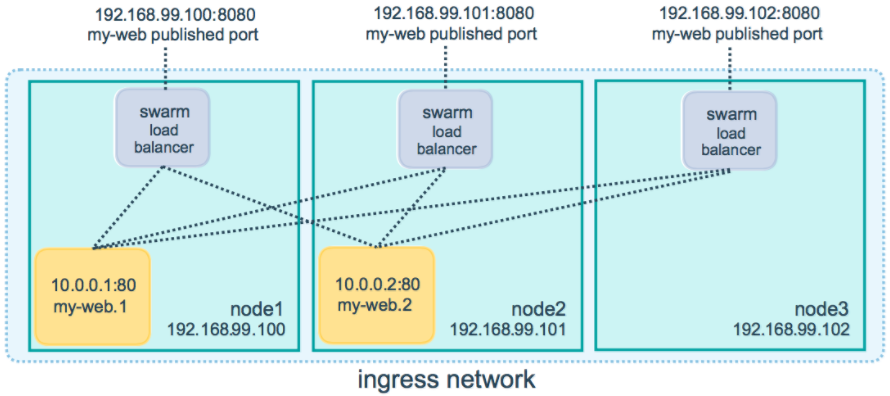
\includegraphics[width=0.7\textwidth]{swarmLoadBalancing.png}
    \attribution{\url{https://www.docker.com}}
\end{center}

Docker Compose + Docker Swarm может использоваться для организации вполне себе настоящей системы распределённых вычислений, и даже довольно производительной, чего может быть вполне достаточно для многих корпоративных информационных систем, хостящихся на серверах компании.

\section{Kubernetes}

% Источник: Cloud Native DevOps with Kubernetes

Для больших высоконагруженных систем с высокими требованиями к надёжности Docker Compose обычно не используется, поскольку он сам по себе относительно мало чего умеет и не очень конфигурируем. Для серьёзных задач применяют несколько более продвинутый оркестратор --- Kubernetes. 

В принципе, задачи у него такие же, как у Docker Compose с Docker Swarm --- имея некоторое количество Docker-контейнеров и некоторое количество машин (физических или виртуальных) в кластере, раскидать контейнеры по машинам, управлять взаимодействием контейнеров, балансировать нагрузку, следить за их временем жизни, запускать/останавливать реплики при необходимости. Kubernetes в разы сложнее в конфигурировании, так что с ним часто используются дополнительные инструменты, упрощающие задачу написания конфигурационных файлов --- это не один docker-compose.yml написать. Однако в разы функциональнее и умнее, поэтому Kubernetes сейчас --- стандарт де-факто для развёртывания больших приложений. 

Интересно, что Docker Desktop имеет встроенную поддержку Kubernetes, так что если у вас есть Docker Desktop, у вас уже есть Kubernetes-кластер из мастер-узла и одного вычислительного узла, который бесполезен для реального развёртывания, но вполне годится для тестирования.

Kubernetes появился в Google из их внутреннего проекта Borg, создававшегося для оркестрации приложений Google. Он с открытым исходным кодом и, раз уж это проект от Google, написан на Go. Причём, Google рекомендует и микросервисы стараться писать на Go, в том числе потому, что типичный размер контейнера с Go-приложением (полного, со всеми слоями) --- порядка шести мегабайт. В отличие от, например, ASP.NET, который, если очень постараться, можно запихать мегабайт в 80. При частых деплоях и огромных кластерах в десятки тысяч машин разница в плане сетевого трафика может быть очень ощутимой.

Архитектурно Kubernetes устроен как довольно обычное распределённое приложение-оркестратор (аналогично Apache Hadoop, например, архитектуру которого показывали в самой первой лекции этого курса). Есть \emph{master}, предоставляющий интерфейс для управления кластером и координирующий действия \emph{node}-ов:

\begin{center}
    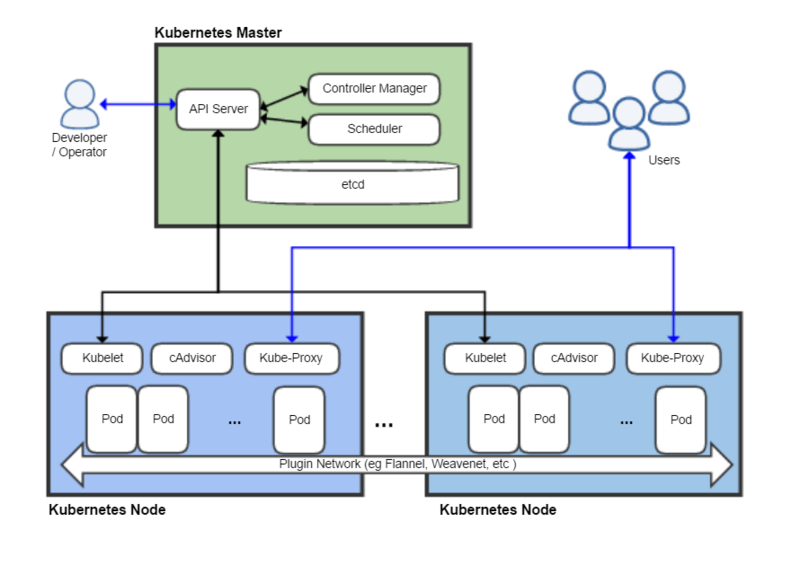
\includegraphics[width=0.8\textwidth]{kubernetesArchitecture.png}
    \attribution{\url{https://ru.wikipedia.org/wiki/Kubernetes}}
\end{center}

Master имеет базу данных конфигурации etcd, где собственно и хранится вся текущая конфигурация системы. Controller Manager отвечает за коммуникацию с облачным провайдером, на котором запущен Kubernetes-кластер, если таковой есть, чтобы использовать его ресурсы типа балансировщиков нагрузки. Scheduler отвечает за раскидывание контейнеров по узлам. Мастер в реальной жизни реплицирован и синхронизируется со всеми репликами, так что в случае отказа одного узла-мастера ничего страшного не случится. Более того, при отказе всех узлов-мастеров приложение, скорее всего, продолжит работать как ни в чём ни бывало.

На каждом из узлов кластера запущены:

\begin{itemize}
    \item Kubelet --- это штука, которая принимает команды от scheduler-а, запускает контейнеры на узле и следит за их статусом;
    \item Kube-Proxy --- компонент, отвечающий за сетевую магию внутри кластера --- маршрутизацию запросов, обработку запросов извне;
    \item cAdvisor --- вообще говоря, не обязателен, это монитор ресурсов, собирает метрики работы контейнера;
    \item Pod --- набор Docker-контейнеров, которые должны работать вместе (например, веб-сервис и его база данных), единица развёртывания в Kubernetes.
\end{itemize}

Конфигурация Kubenetes состоит из \emph{объектов} разных типов, данные о которых хранятся в etcd и попадают туда при применении yaml-файлов с описанием объектов (ну, не обязательно yaml, но суть такая). Вот базовые типы объектов (и структура типичного кластера):

\begin{center}
    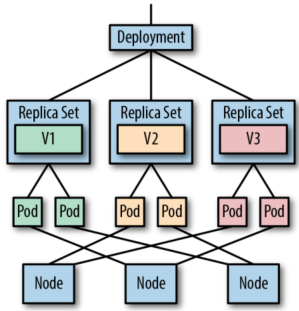
\includegraphics[width=0.4\textwidth]{kubernetesObjects.png}
    \attribution{J. Arundel, J. Domingus, Cloud Native DevOps with Kubernetes}
\end{center}

\begin{itemize}
    \item Deployment --- это описание деплоя одного сервиса (на самом деле, одного Pod-а, то есть по сути группы сервисов). Он управляет запуском контейнеров, репликацией и выкатыванием новых версий. Deployment при создании автоматически создаёт объекты ReplicaSet.
    \item ReplicaSet отвечает за реплицированные группы Pod-ов, запуская и перезапуская их при необходимости.
    \item Pod, как уже говорилось, это набор Docker-контейнеров, работающих вместе, а его описание --- это конфигурация запущенных контейнеров (то, что указывается обычно в docker run --- образ, прокидывание портов, переменные окружения, монтирование папок файловой системы хоста).
\end{itemize}

Вот пример описания простого Deployment-а (манифест):

\begin{minted}{yaml}
apiVersion: apps/v1
kind: Deployment
metadata:
    name: demo
    labels:
        app: demo
spec:
    replicas: 1
    selector:
        matchLabels:
            app: demo
    template:
        metadata:
            labels:
                app: demo
    spec:
        containers:
        - name: demo
            image: cloudnatived/demo:hello
            ports:
            - containerPort: 8888
\end{minted}

\attribution{J. Arundel, J. Domingus, Cloud Native DevOps with Kubernetes}

Тут довольно много всего написано (поэтому для написания таких штук часто используются дополнительные тулы), суть --- в image (образ, который надо запустить) и желаемом количестве реплик (тут одна). Ещё тут активно используется система \emph{меток} --- это просто текстовые строки, которые позволяют проводить выборку нужных ресурсов (например, можно пометить свои ресурсы метками production и test, и применять команды только к ресурсам с указанной меткой).

При выполнении команды kubectl apply -f <имя файла или папки с манифестами> Kubernetes обновит желаемую конфигурацию в etcd, посчитает разницу между текущей и желаемой конфигурацией, и выполнит операции, переводящие текущую конфигурацию в желаемую.

Однако так работать ничего не будет, потому что тут написано, что деплоймент имеет порт 8888, открытый внутри контейнера, но снаружи его не видно. Чтобы было видно, нам потребуется описать ещё один ресурс --- Service. Это прокси и балансировщик нагрузки, который имеет фиксированный ip-адрес и перенаправляет запрос кому-нибудь из реплик:

\begin{center}
    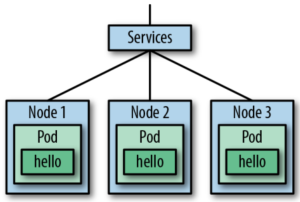
\includegraphics[width=0.4\textwidth]{kubernetesServices.png}
    \attribution{J. Arundel, J. Domingus, Cloud Native DevOps with Kubernetes}
\end{center}

Помимо Service, есть ещё ресурс Ingress, позволяющий более умно маршрутизировать трафик и работать с TLS-сертификатами.

Вот пример описания сервиса:

\begin{minted}{yaml}
apiVersion: v1
kind: Service
metadata:
  name: demo
  labels:
    app: demo
spec:
  ports:
  - port: 9999
    protocol: TCP
    targetPort: 8888
  selector:
    app: demo
    type: ClusterIP
\end{minted}

Этот сервис перенаправляет запросы с порта 9999 хоста на порт 8888 контейнера, а точнее, всех контейнеров с меткой <<demo>> (что указывается в параметре selector).

Теперь, когда у нас есть два манифеста, можно это всё запустить, командами

\begin{minted}{text}
kubectl apply -f k8s/deployment.yaml
kubectl apply -f k8s/service.yaml
kubectl port-forward service/demo 9999:8888
\end{minted}

Полный пример из книги J. Arundel, J. Domingus, Cloud Native DevOps with Kubernetes можно посмотреть у них на GitHub: \url{https://github.com/cloudnativedevops/demo/tree/main/hello-k8s} (дата обращения: 13.12.2021). Причём, можно и запустить --- оно само скачает нужный контейнер с Docker Hub. 

\subsection{Использование Kubernetes}

Первая и главная рекомендация по использованию Kubernetes --- читайте документацию. Про это дело пишут книги (и не одну), так что в маленьком подразделе одной лекции пользоваться Kubernetes не научить (разве что как извращённым способом сделать docker run, как выше). 

Вторая важная рекомендация --- относитесь к конфигурации развёртывания как к коду. kubectl и некоторые другие инструменты умеют писать прямо в etcd, и можно вручную управлять состоянием кластера, вручную меняя количество реплик, порты, ресурсы. А потом в какой-то момент всё упадёт (или вы решите сменить облачного провайдера), вы перезапустите кластер --- и ваша система вообще не работает, потому что вы навносили вручную каких-то изменений и забыли, а сохранённая конфигурация теперь вообще нежизнеспособна. Надо сразу приучаться вносить изменения только декларативно --- пишете/правите манифест, коммитите его в систему контроля версий, применяете (или его за вас применяет CI-система). Так у вас будет всегда актуальный конфиг, и всегда по истории коммитов можно будет найти того несчастного, кто всё сломал, и уволить\footnote{Это основной постулат <<Культуры DevOps>>, о которой в интернете так много общих слов и бессвязных рассуждений --- \emph{во всём виноват программист, бейте его}.}.

\subsection{Контроль состояния контейнера}

Это уже говорилось выше, но для реальных приложений критичен мониторинг. Kubernetes умеет в этом плане довольно многое --- интеграция с cAdvisor, например. Но есть ещё важная штука, которую надо писать руками: livenessProbe. Покажем на примере:

\begin{minted}{yaml}
livenessProbe:
  httpGet:
    path: /healthz
    port: 8888
  initialDelaySeconds: 3
    periodSeconds: 3
\end{minted}

Это часть манифеста Pod или Deployment, в которой написано, что Kubelet, чтобы проверить, жив ли контейнер, должен сделать GET-запрос на URL <ip контейнера>/healthz на порт 8888, и если он ответит с кодом 200, то контейнер жив. Тут также написано, что делать это надо через три секунды после запуска контейнера (чтобы дать ему запуститься) каждые три секунды. Это позволяет детектить ситуации, когда контейнер не упал, но по тем или иным причинам не может исполнять запросы (например, задедлочился).

Есть ещё readinessProbe, устроенная аналогично, но имеющая другую семантику --- что контейнер готов обрабатывать запросы. Если livenessProbe неудачна, контейнер перезапустят, если readinessProbe неудачна, просто не будут направлять ему запросы из Service, а дадут приготовиться к работе.

\subsection{Стратегии обновления}

Ещё в реальной жизни важно обеспечить плавное и аккуратное переключение на новую версию приложения при его обновлении. Для этого есть разные стратегии, самая популярная --- Blue/green deployment. Вместо того, чтобы убить старые контейнеры и запустить новые, создаётся новый набор Deployment-ов, куда выкатывается новая версия, контейнеры внутри инициализируются и готовятся к работе, мы, возможно, вручную тестируем, что всё ок, и переключаем трафик (с помощью Service или Ingress) на них. Делается это через систему меток: добавляем в манифест Service в selector метку deployment: blue, а когда закончим развёртывание второй версии (все ресурсы которой помечены как deployment: green), меняем селектор в Service и применяем его. Дальше по мере окончания работы клиентов с контейнерами в blue-деплойменте можно постепенно отключать контейнеры, пока не останется только green-деплоймент. Либо, если релиз неудачный, одной командой переключиться обратно на старую версию. При релизе следующей версии происходит то же самое, но blue и green меняются местами.

Иногда бывает так, что контейнеры выполняют длительные задачи и деплои происходят чаще, чем одна задача успевает досчитаться (или контейнеры обслуживают длительные подключения, например, через веб-сокеты). Тогда Blue/green deployment обобщается до <<rainbow deployment>> --- когда запущено сразу несколько версий приложения и старые версии постепенно, по мере окончания работы с ними клиентов, выводятся из работы.

А ещё есть Canary deployment --- это когда на новую версию заворачивается некоторый небольшой процент трафика, который постепенно увеличивается, пока не станет 100\%, и тогда старая версия выключается. Это делается для того, чтобы небольшой процент пользователей попробовал новую версию, и если всё плохо и всё упало, то, во-первых, мы бы об этом тут же узнали от средств мониторинга, и во-вторых, пострадал бы только небольшой процент пользователей. Для этого есть даже специальные инструменты, например Istio --- они же, и такая же по сути практика, может использоваться и для A/B-тестирования, о котором наверняка было в курсе по программной инженерии.

Ещё хороший совет --- никогда не используйте тэг latest у Docker-образов, всегда фиксируйте конкретную версию. latest может продвигаться, так что ваша система может меняться незаметно для вас, а если вы используете latest на сторонние образы, вы вообще отдаёте своё приложение на милость сторонним разработчикам, которые могут одной командой всё сломать.

\subsection{Дополнительные инструменты}

Писать манифесты вручную может быть тяжело, а вручную с помощью kubectl следить за состоянием кластера, собирать логи и т.п. может быть вообще невозможно. Поэтому Kubernetes обычно используется с набором инструментов, некоторые из которых независимы, некоторые выросли поверх Kubernetes и используются только для него. Вот некоторые примеры:

\begin{itemize}
    \item Helm --- <<пакетный менеджер>> для Kubernetes, серьёзно упрощающий конфигурирование сторонних приложений внутри вашего кластера. Он же может использоваться как шаблонный генератор манифестов. Управление <<пакетами>> Helm выполняет с помощью Helm Charts --- это шаблон манифестов Kubernetes плюс конфигурационный файл, куда вынесены изменяемые параметры конфигурации, типа портов или меток, которые вставляются в шаблоны манифестов. Пишем Helm Chart один раз, потом применяем сколько угодно раз, просто меняя конфигурационный файл, а не обновляя сотню .yaml-файлов с манифестами ресурсов Kubernetes.
    \item Kubernetes Dashboard --- веб-интерфейс, отображающий статус кластера. Частая ошибка новичков --- делать его доступным без авторизации, несмотря на то, что Kubernetes Dashboard с радостью расскажет все коммерческие тайны и даже секреты, используемые в кластере (логины-пароли, токены и т.д.). Но будучи должным образом защищённым, Kubernetes Dashboard очень удобен для быстрого мониторинга.
    \item Prometheus --- стандарт де-факто для мониторинга и нотификаций, более серьёзная штука, чем Kubernetes Dashboard.
    \item Clair --- сканер контейнеров, статически (то есть без запуска) проверяет их на часто встречающиеся уязвимости. В реальной жизни стоит всегда прогонять Clair или что-то такое на контейнерах, деплоящихся в кластер, чтобы вас не сломали.
    \item Velero --- инструмент для бэкапа состояния кластера (в частности, делать бэкап etcd).
\end{itemize}

\subsection{Стратегии мониторинга}

Помимо инструментов для сбора метрик, важно также определиться с самими метриками. выше говорилось, что это некоторое искусство, однако есть типовые паттерны:

\begin{itemize}
    \item Requests-Errors-Duration (RED) --- число входящих запросов, число ошибок и продолжительность выполнения каждого запроса.
    \item Utilization-Saturation-Errors (USE) --- использование аппаратных ресурсов (процессора, памяти, диска), длина буфера входящих запросов, ждущих обработки, число ошибок.
\end{itemize}

RED больше про внешнее поведение сервиса, USE больше про его внутреннее состояние. Поэтому RED полезен как показатель общего здоровья и использования системы, USE позволяет понять, насколько эффективно приложение использует выделенные ему мощности (что может помочь оптимизировать стоимость аренды ресурсов).

\section{Облачная инфраструктура}

Из всего вышесказанного может сложиться впечатление, что чтобы содержать распределённое приложение, вам потребуется купить высокопроизводительный кластер или суперкомпьютер, или, если приложение маленькое, поставить дома/в офисе в угол какой-нибудь ненужный ноут, пробросить на него порты и запустить там узел Kubernetes. Это впечатление неправильное. Практика показывает, что самим содержать вычислительные ресурсы для работы большого приложения может быть гораздо накладнее, чем само приложение. А если приложение маленькое и работает на ноуте в углу, то, скорее всего, не защищено от выключения электричества, пропажи интернет-соединения или порчи жёсткого диска. В любом случае это плохая идея, и лучше уж разориться на аренду облачных ресурсов у компаний, которые на этом специализируются, и предоставляют по заказу высокопроизводительную и надёжную инфраструктуру.

Единственное, что предоставляют они уж очень много чего, и если вы решите пойти, например, на сайт AWS с мыслью арендовать небольшую машину, где можно было бы запустить Docker-контейнер с вашим веб-приложением, вы можете сойти с ума (хотя бы от сотни разных трёхбуквенных аббревиатур на главной странице). Вообще, облачные сервисы делятся на три крупные категории:

\begin{itemize}
    \item Infrastructure as a Service --- когда облачный провайдер предоставляет вам виртуальную машину, дисковое пространство и некоторое количество сетевого трафика, дальше делайте что хотите. Например, ставите на виртуалку Docker, настраиваете на нескольких виртуалках Kubernetes-кластер и т.д.
    \item Platform as a Service --- когда облачный провайдер предоставляет набор уже готовых сервисов, которые вы можете использовать, например, Kubernetes-кластер, который вы инструментами облачного провайдера конфигурируете и запускаете на нём свои контейнеры, даже не зная, на какой операционной системе они там работают. Обычно дешевле и быстрее в настройке, чем IaaS, но если вы знаете, что делаете. Если не знаете, количество опций типа балансировщиков нагрузок, хранилищ данных и т.п. может вогнать в депрессию.
    \item Software as a Service --- когда облачный провайдер предоставляет уже готовое приложение (например Google Docs или облачные IDEшки).
\end{itemize}

В принципе, разные виды сервисов можно смешивать в каких угодно пропорциях, собирая инфраструктуру под своё приложение. Полноценные виртуальные машины могут использовать уже преднастроенные облачным провайдером сервера СУБД и общаться с Docker-контейнерами, развёрнутыми в PaaS-стиле.

Вот наиболее популярные облачные провайдеры. Они все имеют более-менее одно и то же, все в том или ином виде предоставляя возможности по запуску приложений, поддержку оркестрации (Kubernetes или Docker Compose только недавно начали своё победное шествие, многие провайдеры всё ещё имеют свои проприетарные оркестраторы, типа Heroku --- нестандартно, зато очень удобно). 

\begin{itemize}
    \item Amazon Web Services --- мировой лидер в облачной инфраструктуре, ему принадлежит почти 50\% рынка (хотя на этом рынке очень большая конкуренция, потому что кто владеет облачной инфраструктурой, тот владеет миром). Инфраструктура Amazon географически разнесена и весьма надёжна --- они гордятся тем, что система будет работать даже при одновременном подрыве более 30 ядерных боеголовок.
    \item Microsoft Azure --- то же самое от Microsoft, популярна в основном потому, что хорошо интегрирована с инструментами разработки от Microsoft. Некоторое время была недоступна в России (из-за санкций?), но сейчас (на декабрь 2021 года) всё работает.
    \item Google Cloud --- в Google разработали Kubernetes, поэтому Google Kubernetes Engine (часть Google Cloud) --- старейший и наиболее зрелый провайдер для кластеров Kubernetes. Больше ничем особо не примечателен (разве что Google Colab --- позволяет погонять свой ненужный ML на настоящих дорогих видеокартах бесплатно для студентов).
    \item Всё остальное, среди которого стоит, наверное, отметить Yandex.Cloud --- по российскому закону о персональных данных их надо хранить на территории России, а крупные облачные провайдеры в России дата-центров всё ещё не имеют. Yandex.Cloud got you covered. Ну и, наверное, заслуживает упоминания Heroku, как очень дружественная к новичкам платформа.
\end{itemize}

\subsection{Экосистема AWS}

В качестве примера типичного облачного провайдера рассмотрим Amazon Web Services. Вот что он умеет (в частности --- так-то он умеет ещё сотни всего):

\begin{itemize}
    \item Вычисления:
    \begin{itemize}
        \item EC2 (Elastic Compute Cloud) --- аренда виртуалок.
        \item ECS (Elastic Container Service) --- среда для запуска Docker-контейнеров, интегрированная с Amazon Elastic Container Registry (типа Docker Hub, но на Amazon). Свой оркестратор.
    \end{itemize}
    \item Сеть:
    \begin{itemize}
        \item VPC (Virtual Private Cloud) --- конфигурируемая виртуальная сеть, с настройками подсетей, разделением по регионам и т.п.
        \item ELB (Elastic Load Balancing) --- продвинутый балансировщик нагрузки.
        \item API Gateway --- ну, API Gateway, как в описании микросервисного стиля.
    \end{itemize}
    \item Устройства хранения:
    \begin{itemize}
        \item EFS (Elastic File System) --- распределённая масштабируемая файловая система, монтируется в виртуалку или контейнер как фактически ещё один диск.
        \item EBS (Elastic Block Store) --- фактически, облачный жёсткий диск.
    \end{itemize}
    \item SaaS, базы данных:
    \begin{itemize}
        \item RDS (Relational Database Service) --- предустановленные сервера СУБД (внутри может быть много чего, от MariaDB до Oracle).
        \item DynamoDB --- облачная NoSQL-база от Amazon.
        \item OpenSearch Service --- поисковый движок и анализатор слабоструктурированных и неструктурированных данных (в т.ч. логов, часть Elastic Stack).
    \end{itemize}
\end{itemize}

\subsection{Инфраструктура как код}

Теперь понятно, что вручную сидеть и прокликивать сотни окошек в Amazon Web Services, деплоя пятьдесят разных сервисов и <<обвязку>> к ним может быть очень хлопотно, а если мы вдруг захотим перейти на Azure, то для большого приложения проще сразу самоубиться. Поэтому все нормальные облачные провайдеры поддерживают веб-API для конфигурирования инфраструктуры, и этим пользуется подход Infrastructure as Code. Kubernetes использует подход <<Конфигурация развёртывания как код>>, описывая в манифестах развёртывание контейнеров на уже готовой инфраструктуре, подход IaC идёт дальше и предлагает описывать как код саму инфраструктуру: 

\emph{<<The enabling idea of infrastructure as a code is that systems and devices which are used to run software can be treated as if they, themselves, are software>> (Infrastructure as Code, Kief Morris)}

Модель требуемой инфраструктуры описывается независимым от облачного провайдера образом (в духе <<надо кластер Kubernetes с пятью узлами, балансировщик нагрузки и сервер NoSQL-СУБД>>), коммитится в систему контроля версий и применяется относительно выбранного облачного провайдера (и тогда кластер Kubernetes конфигурируется из имеющихся у провайдера ресурсов). Это позволяет, во-первых, иметь воспроизводимое развёртывание (в идеале, с почти нуля --- вам всё-таки потребуется завести аккаунт и привязать банковскую карту), во-вторых, перейти на другого облачного провайдера одной командой (в идеале).

Пример такого инструмента --- Terraform. Поддерживает что-то около 135 облачных провайдеров, имеет консольный интерфейс, который позволяет залогиниться в выбранный облачный провайдер (например, Microsoft Azure) и применить желаемую конфигурацию. Например, вот конфигурация Kubernetes-кластера для Azure (из туториала \url{https://learn.hashicorp.com/tutorials/terraform/aks?in=terraform/kubernetes}):

\begin{minted}{text}
resource "azurerm_kubernetes_cluster" "default" {
    name                = "${random_pet.prefix.id}-aks"
    location            = azurerm_resource_group.default.location
    resource_group_name = azurerm_resource_group.default.name
    dns_prefix          = "${random_pet.prefix.id}-k8s"
    
    default_node_pool {
        name            = "default"
        node_count      = 2
        vm_size         = "Standard_D2_v2"
        os_disk_size_gb = 30
    }
    
    service_principal {
        client_id     = var.appId
        client_secret = var.password
    }
    
    role_based_access_control {
        enabled = true
    }
    
    tags = {
        environment = "Demo"
    }
}
\end{minted}

Специфика конкретного провайдера, увы, необходима --- например, предоставляемые ресурсы называются у разных провайдеров по-разному, но подредактировать один файл всё равно проще, чем копаться в GUI облачных провайдеров вручную.

\end{document}